% \pagebreak[4]
% \hspace*{1cm}
% \pagebreak[4]
% \hspace*{1cm}
% \pagebreak[4]
\chapter{Literature Review}
%\ifpdf
%    \graphicspath{{Literature/LiteratureFigs/PNG/}{Literature/LiteratureFigs/PDF/}{Literature/LiteratureFigs/}}
%\else
%    \graphicspath{{Literature/LiteratureFigs/EPS/}{Literature/LiteratureFigs/}}
%\fi



Paul Ehrlich famous quote is, �To err is human, but to really foul things up you need a computer�. Since the programmers are ordinary human beings, it is most obvious that some errors remain in the software after its completion. Errors are not tolerated as they can cause great loss. According to the National Institute of Standard and Technology 2002, 10 report, software errors cost an estimated \$59.5 billion loss to US economy annually. The destruction of the Mariner 1 rocket (1962) that cost \$18.5 million was due to a simple formula coded incorrectly by a programmer. The Hartford Coliseum Collapse (1978) costing \$70 million, Wall Street crash (1987) costing \$500 billion, Failing of long division by Pentium (1993) costing \$475 million, Ariane 5 Rocket disaster costing \$500 million and many others are caused by minor errors in the software. To achieve high quality, the software has to satisfy rigorous stages of testing. The more complex and critical the software, the higher the requirements for software testing and the larger the damage caused if the bug remains in the software. 


\section{Software Testing}
In the IEEE standard glossary of software engineering terminology \cite{american1984}, testing is defined as the process of exercising or evaluating a system or system component by manual or automated means to verify that it satisfies specified requirements and actual results. Test is more successful if it finds more errors in the software. Once errors are found in the SUT, the software is given back to the developers for removing the found errors and after rectifying the mentioned errors the software is again handed over to the testers for retesting. The testing process starts from the very beginning of software development and remains continuos throughout the life of the software.

One thing to keep in mind is that �program testing can be used to show the presence of bugs, but never to show the absence of bugs� \cite{Dijkstra1972}. Which means SUT that passes all the tests without giving a single error is not guaranteed to contain no error. The testing process increase however the reliability and confidence of the users in the tested product.

\subsection{Software Test Plan}
As proper planning is the key to success for many projects this is often also true with software testing. A software test plan is a well defined document that defines the goal, scope, method, resources and time schedule of the testing.

\subsection{Software Testing Approaches}
The testing process starts from the very beginning of the System Development Life Cycle (SDLC) and is carried out in the following two ways.

\begin{enumerate}
\item Static Testing 
\item Dynamic Testing
\end{enumerate}

\subsection{Static Testing}

The term static means �still� or �non executable�. Static Testing is the process in which software documentation/source code is checked for errors without any execution. All high quality software�s will always be accompanied by documentation in addition to software code. These include requirements, de- sign, technical, end user and marketing documentation. Reviews, walkthroughs or inspections are most commonly used for static tests.
For instance it is necessary to do the static testing of user documentation for errors because software developed at the cost of millions of dollars have been neglected and abandoned for the only reason that end users were not able to find out the proper way to operate it to do their routine business. Users tend not to think �I will figure out how to operate this software�; rather, they say, �this software doesn�t do what I need it to do, so I want the old system back� \cite{Everett2007}.

\subsection{Dynamic Testing}

Dynamic means �variable� or �changeable� so Dynamic Testing is the process in which software code is executed and input is converted into output through processing. Results are analysed to find any error in the software. It is not necessary that dynamic testing start once the software is fully complete. Instead it can start from a single method/unit. Unit testing, integration testing, system testing, and acceptance test- ing are most commonly used as dynamic testing methods. Dynamic testing can be manual or automated. In manual testing the programmer develops the test cases which are executed by the developed software to find any error in processing or output. Similarly in automated testing the software or components of the software is given as input to testing software that automatically generates test cases and executes the SUT against them to find any errors. Manual testing typically consumes more time and resources than automated testing.


\subsection{Methods of Dynamic Software Testing}
There are three methods for testing the software dynamically.

\begin{enumerate}
\item Black-Box Testing
\item White-Box Testing
\item Grey-Box Testing
\end{enumerate}

\subsubsection{Black-Box Testing}
Black-Box or Functional testing is the method in which the testers don�t know about the structure of the software. Test cases are derived from the specifications of the SUT and tests pass only if the output checks, according to the specification no matter how it is internally processed by the software. The main emphasis of black-box testing is to check the functionality of the product.

\subsubsection{White-Box Testing}
White-Box or Structural testing is a method in which the testers must know about the complete structure of the software. Test cases are derived from the code structure of the SUT and the test is pass only if the results are correct according to the specification as well as the execution is carried out according to oracle. The main emphasis of the white-box testing is not only functionality but also code coverage \cite{Agarwal2009}.

\subsubsection{Grey-Box Testing}
Grey-Box testing is the combination of both black-box/functionality and white-box/structural testing. The tester knows about both the functionality and the internal structure of the SUT. Some of the test cases are based on the functionality and some of the test cases are based on the structure. Emphasis of grey-box testing is both on code coverage as well as functionality \cite{Savenkov2008}.

\subsection{Software Testing Workflow}
There are many software techniques like unit testing, integration testing, random testing, regression testing, system testing, acceptance testing, performance testing, load testing, stress testing, alpha testing, beta test etc. All testing techniques belong to black-box, white-box or grey-box approach. Each testing technique has its own strength and weaknesses but the technique in focus here is Random Testing.


\begin{figure}[h]
\begin{center}
	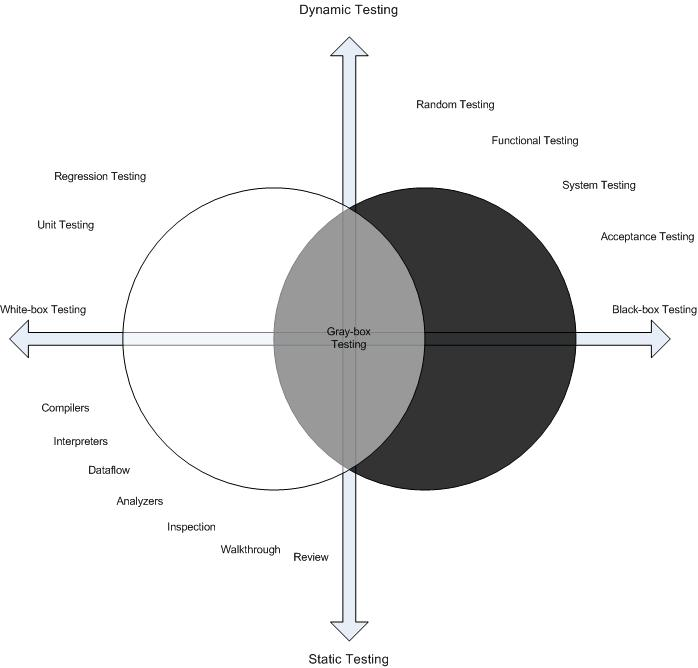
\includegraphics[width=16cm, height=12cm ]{Literature/Drawing34.jpg}
	\caption{Software Testing Workflow}
\end{center}  
\end{figure}


We have explained software testing graphically with the help of plotting venn diagram on two dimensional axis. The positive x axis represent black-box while negative x axis represent white-box testing. Grey-box testing in the middle is represented by the overlapping of black-box and white-box testing. Similarly on positive y axis we have dynamic testing and on negative y axis we have static testing.
Now if a test is black box and dynamic then the test will fall in 0 to 90 degree on the diagram and if the test is black-box and static then it will fall in 270 to 360 degree. On the other hand if the test is white-box and dynamic then it will fall in 90 to 180 degree and if the test is white-box and static then it will fall in 180 to 270 degrees.

\subsection{Manual Testing}
 A software testing technique to find faults in a class or group of related classes, such that the tester must write the code by hand to create test cases and test oracle \cite{Ciupa2008}. While manual testing is effective in some cases, in general, it is a laborious, time consuming, error-prone \cite{tretmans1999}. It further requires testers to have appropriate skills, experience and in depth knowledge of the under test software in order to evaluate it from different perspectives.
 
\subsection{Automated Testing}
A software testing technique to find faults in a class or group of related classes, such that the test cases and test oracle is generated automatically by a testing tool \cite{Leitner2007}. The tools can automate part of a test i.e. generation of test cases, execution of test cases and evaluation of results or the whole test process. The use of automated testing made it possible to test large volumes of code that would be otherwise impossible \cite{ramamoorthy1975}.

\subsubsection{Exhaustive Testing}
A software testing technique in which a software is tested with all possible combination of inputs. This technique can prove conclusively that the software meet its specification however exhaustive testing is seldom feasible because of the large input domain or too many paths in a software code. Testers therefore are usually only able to use a small portion of a program�s input domain to test a given software \cite{chan2003normalized}.


%\section{Automated Random Testing}
%\subsection{Test Data Generation}
%\subsection{Test Execution}
%\subsection{Test Oracle}
%\subsection{Test Report}

\subsubsection{Random Testing}
Random testing is a dynamic and black-box testing approach in which the software under test is tested by selecting random test cases from already specified input domain \cite{Chan2002}. The input domain is the set of all possible inputs to the software and the number of test cases selected are dependent on the basis of desired reliability or available resources.

\begin{figure}[h]
	\centering
	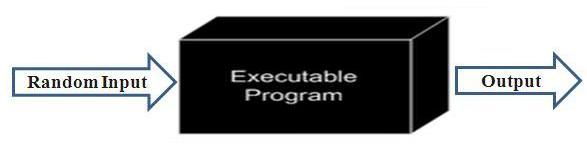
\includegraphics[scale=0.5]{Literature/figure1.jpg}
	\caption{Random Testing}
  
\end{figure}

According to Richard Hamlet \cite{Hamlet1994}, to conduct random testing, we need to define an input domain, then we take test points randomly from the whole input domain through a random number/test case generator independently without any restrictions. The program under test is executed on these points and the results obtained are compared to the program specifications. The test fails if any input leads to incorrect results or otherwise it is successful. The internal working of random testing is described in figure 1.2.


\section{Variations in Random Testing}
Different researchers tried various strategies to improve the performance of random testing. In order to better understand the topic we have studied each strategy in detail.

\subsection{Adaptive Random Testing}
Adaptive random testing (ART) \cite{Chen2008} is based on the existence of failure patterns across the input domain detected by Chan et al \cite{Chan1996}. They observed that failure inducing inputs in the whole input domain form certain geometrical patterns. They divided these patterns into point, block and strip fault patterns. Each one is described below.

\begin{figure}[h]
	\centering
	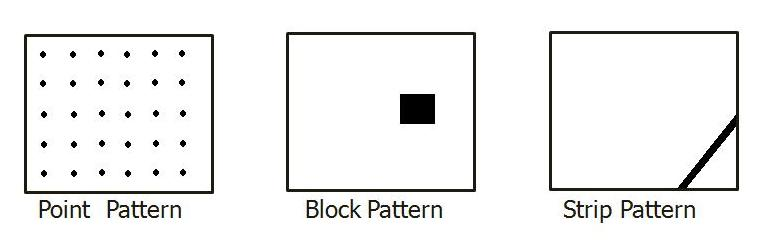
\includegraphics[scale=0.5]{Literature/pointblockstrip}
	\caption{Patterns of failure causing inputs}
	\label{fig:patterns}
\end{figure}

In the figure \ref{fig:patterns} the square box indicates the whole input domain. The white space shows legitimate or faultless values while the black colour points, block and strip inside each box indicate the point, block and strip fault patterns in the input domain.

\begin{enumerate}
\item Point pattern: In the point pattern failure inducing inputs are scattered across the input domain in the form of stand-alone points. Example of point pattern is the division by zero in a statement total = num1/num2; where num1, num2 and total are variables of type integer. 
\item Block pattern: In the block pattern multiple failure inducing inputs lies in a close vicinity to form a block in the input domain. Example of block pattern is failure caused by a statement if ( (num \textgreater 10) \&\& (num \textless 20) ). Here 11 to 19 is a block of faults.
\item Strip pattern: In the strip pattern the failure inducing inputs form a strip across the input domain. Example of strip pattern is failure caused by a statement num1 + num2 = 20. Here multiple values of num1 and num2 can lead to the fault value 20.
\end{enumerate}

The authors argued that ordinary random testing may generate test inputs lurking too close or too far from the fault inducing input and thus failing to discover it. To generate more fault targeted test inputs they suggested ART. ART is a modified version of ordinary random testing where test values are selected at random like before but evenly spread across the input domain. To achieve an even distribution of test cases across the input domain they used two sets. The executed set having the test cases that have been executed by the system and the candidate set that contain the random selected test cases from the bounded input domain as candidates for execution. Initially both the sets are kept empty. The first test case is selected at random from the candidate set and stored in executed set after execution, the second test case is then selected from the candidate set based on the criteria that it is far away from the last executed test case. Thus the whole input domain can be tested and their are more chances of generating test input from inside of the existing geometrical patterns. 

In the experiments they used number of test cases required to detect first failure (F-measure) as a performance matrix instead of the traditional matrix i.e. probability of detecting at least one failure (P-measure) and expected number of failures detected (E-measure). Results of the experiments performed on published programs using ART showed up to 50\% increase in the performance of than ordinary random testing. Results showed significant improvement, however, the issues of increase overhead, spreading test cases across the input domain for complex objects and efficient ways of selecting candidate test cases still exist. Chen et al evolve their work on ART to address some of these issues in \cite{chen2009enhanced} and \cite{Chen2005}. 

\subsection{Mirror Adaptive Random Testing}
As discussed in the above section ART provide better results, however the increase in overhead due to extra computation to achieve even spread of test inputs makes it less cost effective. Mirror Adaptive Random Testing (MART) \cite{Chen2003} is an innovative approach that uses mirror partitioning technique to reduce the overhead of ART by decreasing the extra computation involved in ART.

\begin{figure}[h]
\begin{center}
	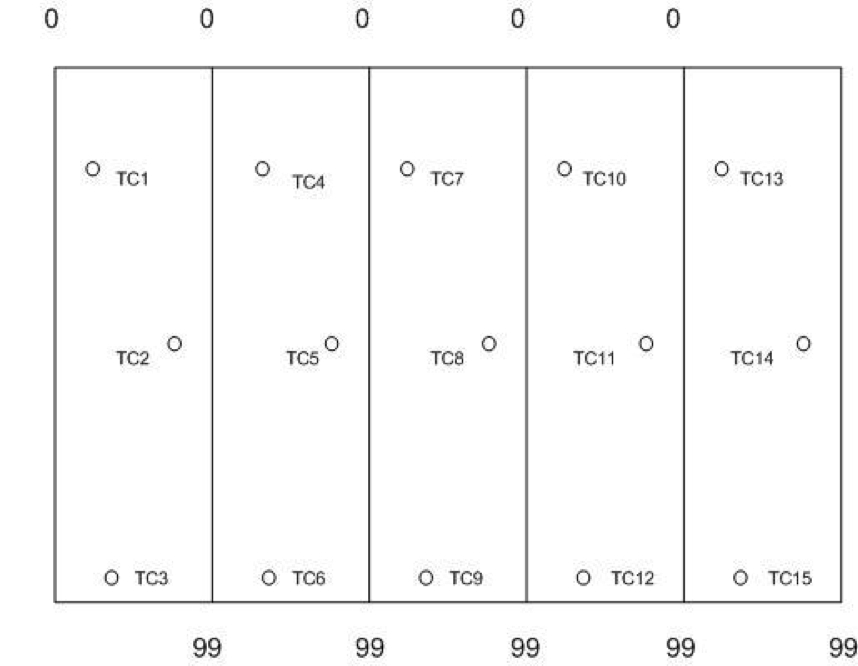
\includegraphics[width=10cm, height=7cm ]{Literature/mat}
	\caption{Mirror Adaptive Random Testing (0-500)}
\end{center}  
\end{figure}

In this technique, the input domain of the program under test is divided into n disjoint subdomains of equal size and shape. One of the subdomain is called source subdomain while all the others are termed as mirror subdomains. ART is then applied only to the source subdomain to select the test cases and from all other subdomains test cases are selected by using mirror function. In MART \{(0, 0), (u, v)\} are used to represent the whole input domain where (0, 0) are the leftmost and (u, v) are the rightmost top corner of the two dimensional rectangle. On splitting it into two subdomains we get \{(0, 0), (u/2, v)\} as source subdomain and \{(u/2, 0), (u, v)\} as mirror subdomain. Let suppose we get x and y test cases by applying ART to source subdomain, now we can linearly translate these test cases to achieve the mirrored effect, i.e. (x + (u/2), y) as shown in the figure ???. Experimental results showed that the performance of MART is equal to ART with MART using only one quarter of the calculations of that of ART.    



\subsection{Directed Automated Random Testing}


\subsection{Quasi Random Testing}
Quasi-random testing \cite{Chen2005} is a technique developed to obtain an even better distribution of test cases across the input domain in less computation time with respect to ART. From various experiments Chen et al found out that the failure causing inputs not only form specific pattern but these patterns are continuous as well. Quasi-random testing don't restrict random selection of test cases like ART or RRT rather it uses a class with a formula. This formula forms an s-dimensional cube in s-dimensional input domain and produces number with Quasi sequence (a sequence of numbers that have small discrepancy and low dispersion) for an s-dimensional input domain. These sequence of numbers are then used by the Quasi approach to select the test cases from s-dimensional input domain. For performance analysis the author compared Quasi approach with ART and random testing. Results showed that the approach is better than random testing but not than ART.

%\subsection{Monti Carlo Random Testing}

%\subsection{Good Random Testing}

\subsection{Feedback-directed Random Test Generation}
In a bid to improve random testing Pacheco et al., \cite{Pacheco2007} developed a technique which produces unit tests randomly for object oriented programs which are later used for testing the units of the SUT. It is an incremental approach in which unit tests are created and executed against a set of contracts and filters. The feedback obtained from this execution serve as a basis for a sequence of new unit tests. The feedback of the unit test indicate that it is useful to create new input but if it is redundant or illegal like it throws IllegalArgumentEexception error then they are discarded and no unit test of similar nature is created based on its feedback. Thus it only selects unit tests which can be effective in finding bugs or can be used for regression testing.
Results of the experiments adopting the technique of Feedback-directed random test generation shows that it can be more productive in code coverage and error detection than systematic and undirected random test generation.

\subsection{Randoop: Feedback-directed Random Testing}
Randoop stands for RANdom tester for Object Oriented Programs \cite{Pacheco2007b}. It tests software by using the principle of feedback-directed random test generation to produce unit tests for java and .NET. Randoop�s input is a set of classes that is to be tested within a certain time and optionally a set of contracts that extend the existing default contracts. After processing the input according to the method of feedback-directed random testing it give two test suites as output. One is contract voilating tests and the other is regression tests.

%\subsection{Adaptive Random Testing for Object-Oriented}



\subsubsection{Object Distance and its application}
To improve the performance of random testing the emphasis of ART was on the distance between the test cases. But this distance was defined only for primitive data types like integers and other elementary input. Ciupa et al defined the parameters that can be used to calculate distance between the composite programmer-defined types so that ART can be applicable to testing of todays object-oriented programs \cite{Ciupa2006}. Two objects have more distance between them if they have more dissimilar properties.
The parameters to specify the distance between the objects are dynamic types, values of its primitive and reference fields. Strings are treated as a directly usable values and Levenshtein distance \cite{Levenshtein1966} which is also known as edit distance is used as a distance criteria between the two strings.
To implement object distance first all the distances of the objects are measured. Then two sets candidate- objects containing the all the objects ready to be run by the system and the used-objects set which is initially empty. First object is selected randomly from the candidate-object set and is moved to used- object set when executed by the system. Now the second object selected from the candidate set for execution is the one with the biggest distance from the last executed object present in the used-object set. This process is continue until the bug is found or the objects in the candidate-object set are finished.

\subsubsection{ARTOO Tool}
After the criteria to calculate the distance between the objects is defined \cite{Ciupa2006}, the same team implemented that model and performed several experiments to evaluate the proposed model. Adaptive Random Testing for Object Oriented (ARTOO) is a testing strategy, based on object distance, implemented in AutoTest tool [16].
ARTOO was implemented as a plug-in strategy in AutoTest. It only deals with creating and selecting inputs and all other functionality of the AutoTest was the same. Since ARTOO is based on object distance therefore the method for test input selection is to pick that object from the candidate set (A pool of objects that is a potential candidate to be executed by the system) which has the highest average distance in comparison to the objects already executed.
In the experiments classes from EiffelBase library [17] were used. To evaluate ARTOO the same tests were also applied to directed random strategy (RAND). The outcome of the experiments showed that ARTOO finds the first bug with fewer test cases than RAND. The computation to select test case in ARTOO is more than RAND and therefore ARTOO takes more time to generate a test input. The experiments also found few of the bug found by ARTOO were not pointed out by RAND furthermore ARTOO is less sensitive to the variation of seed value than RAND.

\subsubsection{Experimental Assessment of Random Testing for Object-Oriented Software}
In this research the effect of various parameters involved in random testing and its effect on efficiency is evaluated by performing various experiments on Industrial-grade code base.
Large scale clusters of computers were used for 1500 hours of CPU time which resulted in 1875 test sessions for 8 classes under test. \cite{Ciupa2007} The finding of the experiments are
1. Version of random testing algorithm that is efficient for smaller testing timeout is equally efficient for higher testing timeouts.
2. The value of seed for random testing algorithm plays a vital role in finding the number of bugs in specific time.
3. Most of the bugs are found in the first few minutes of the testing sessions.


\subsection{Restricted Random Testing}
Motivated from Adaptive random testing, aim of Restricted Random Testing (RRT) is the same that is selection of test cases from the input domain such that the whole input domain is represented [?]. The plan to achieve an even selection of test cases from the input domain is accomplished by forming an exclusion zone around the first random selected test case.

\begin{figure}[h]
	\centering
	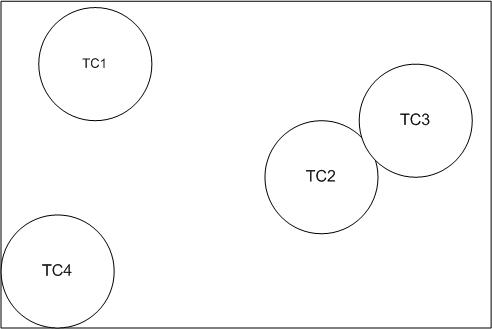
\includegraphics[scale=0.5]{Literature/RRT}
	\caption{Input domain with exclusion zone around the selected test case}
\end{figure}

The next random test case then must be selected outside of this exclusion zone. It makes sure that there is enough distance between the two test cases. The exclusion zone is fixed around each test case and the area of each zone decreases with successive cases.
Experimental results of seven error seeded program indicated that RRT is 55\% more effective than ordianry/undirected random testing in terms of f-measure (Where f-measure is the total number of test cases required to find the first failure).

%\section{Automated Random Testing Tools}

\subsection{JCrasher}
JCrasher is an automatic testing tool that uses a random testing technique to test java classes/programs \cite{Pacheco2007b}. The main features of JCrasher are:
1. The randomly created test cases are according to the type and parameters of the methods under test.
2. It uses special heuristics rules, after the execution of the test cases, to see whether the given excep- tions are real bugs or the generated input violated the pre-conditions of the program.
3. To clarify the testing from any old tests JCrasher make it sure that every test run on a clean state.
4. JCrasher also produces test cases for JUnit that can be integrated into IDEs like Eclipse.
To use JCrasher we have to supply set of Java classes in byte code and testing time. JCrasher analyzes the classes and create test cases randomly with the same type and same parameter list. These test cases are only for public methods of the classes and they check for any system crash. List of exceptions is obtained as a result of execution of test cases which are differentiated as bugs and precondition violations by the input.

\subsection{JArtage}
Jartege (JAwa Random TEst GEnerator) is a tool that randomly generates unit tests for classes specified with JML (Java Modeling Language) \cite{Oriat2004}. The specification of Java classes with JML serves two pur- poses. First, all the test cases generated by Jartege have to verify the conditions defined by JML and thus irrelevant test cases are eliminated. Secondly these JML specifications are also used as oracles. Apart from the JML specification which are made by hand it automates the whole testing process which include test case generation, execution, comparing it against oracle and using the generated test cases for future regression testing.

\subsection{Eclat}
Eclat \cite{Pacheco2005} is a tool that automatically generates unit tests for Java. Eclat can be executed from both command line or from IDE where it can be installed as a plug-in. [28]. Eclat selects a sub-set of test inputs from a large domain, that is likely to reveal fault in the SUT. Eclat takes a correct execution of the SUT and on the basis of it creates an operational model. It then selects only these test inputs from the input domain which fail to comply with the model. A Reducer function removes the redundant test inputs and the remaining test inputs are likely to discover faults in the SUT. Based on the operational model it also produces an automated oracle. Various experiments results shows that Eclats is very effective in finding faults and the ratio of finding faults and test inputs is almost same.

\subsection{JTest}
Parasoft Jtest is a commercial tool that automatically generates and execute unit tests. It can be easily integrated to Java IDEs like Eclipse where it provide two main functionalities, i.e. Static Analysis, Unit testing and code coverage. [25]
In static analysis Jtest takes a complete project or set of classes as input and compares it with a list of built-in rules. The statement violating any of these rules is an error. It also suggests probable fixes for the detected fault.
For unit testing it takes a class as an input and processes a number of scenarios against it to generate and execute unit tests. Once unit tests are executed they become the part of regression test for future reference.
Jtest also shows the code coverage of the program by colour coding the statements that are not executed by the unit tests.

\subsection{QuickCheck}
QuickCheck \cite{Claessen2000} is a light weight random testing tool that is developed specifically for testing of Haskell programs \cite{Hudak2007}. Haskell is a functional programming language where programs are evaluated using expressions rather than statements as in case of imperative programming. Therefore in this process the tester defines certain expressions for the functions that must hold for a large number of test cases to be correct. These test cases are generated automatically through generator function which can be set by the tester to generate random test cases or according to specific criteria. After processing all the generated test cases any test case that causes the expression to become false is considered faults.

\subsection{AgitarOne}
AgitarOne is a commercial tool that automatically generates unit tests. It has a Junit Generator engine that can create 25,000 lines or more of Junit per hour [29]. It can be easily integrated into famous IDE like Eclipse. It takes as input, classes under test, time and optionally any knowledge or test cases that has a positive influence on the performance of the testing process. The generated Junit tests can be run from the same IDE and can also be used for later regression testing. The GUI interface is called a dashboard which provides in depth knowledge of the tests conducted, failures detected, alerts and the archieves of the tests conducted earlier. It also shows the coverage obtained after executing the Junits against the code under test.

\subsection{Autotost}
Based on Formal Automated testing AutoTest is a tool used for testing of Eiffel programs \cite{Ciupa2007}. The Eiffel language use the concept of contracts (pre-conditions, postconditions and class invariants). Input can be a single class, method or a set of classes which is then processed by AutoTest to generate test cases. It generates both primitive and object type test cases. All the generated test cases are kept in a pool and then randomly a test case is selected from it for execution. A user can set the features of the AutoTest options include: Number of test cases to generate, whether to monitor pre or post condition, order of testing and the initial values of the primitives variables.

\subsection{TestEra}
TestEra \cite{Khurshid2004} is a novel framework for testing Java applications. All the tests are produced and executed in an automated fashion. Tests are conducted on the basis of the method specifications \cite{Chang1999}. TestEra takes methods specifications, integer value as a limit to the generated test cases and the method under test. It uses pre-conditions of a method from specifications to automatically generate test cases up to the specified limit. These test cases are then executed on the method and the result is compared against the postconditions (oracle) of that method. Any test case that fails to satisfy postcondition is considered as a fault. The complete error log is displayed in the Graphical User Inteface (GUI).

\subsection{Korat}
Korat \cite{Boyapati2002} is an automated testing tool for Java programs that generates and execute test cases for a method based on its formal specification. To generate test cases for a method Korat makes use of its pre-condition. It then executes the generated test cases against the method specifications. Korat uses JML for specifications. In order to generate test cases for a method Korat constructs new methods that return a Boolean value (Java Predicate) from its pre-conditions. When given these Java predicates Korat generates all non isomorphic input for which the return value of predicate is true. To check correctness of the method, Korat executes the test cases on that method and analyzes the output with the post conditions of the method (oracle). A fault in a method under test throws an exception to indicate the violation of the post-condition.

\subsection{YETI}
The final tool we discuss is YETI (the York Extensible Testing Infrastructure) [33], which is entirely automated and freely available as open-source. It can be used for testing programs written in Java, JML, C, command-line and .Net \cite{Oriol2010c}. It can also be run in cloud for faster execution \cite{Oriol2010}. It is implemented in Java and uses random technique for testing. It has GUI which makes it easy to diagnose problems at runtime. It is able to call up to one million calls per minute on Java code. YETI oracle is language dependant. If the specifications are available, YETI checks the code against the specifications for any inconsistency. In case of programs having assertions YETI interprets violations as failures and in case there is no specifications or assertions, YETI performs robustness testing and considers undeclared run- time exceptions as faults. Errors-revealing test cases are reproduced at the end of each testing session. Experiments conducted with YETI showed significant number of bugs in Java.lang class (45 faults) and Itext (120 faults).

\subsection{Tools for Automated Random Testing}
From the literature we can find a number of open source and commercial testing tools that automatically generate unit tests. Each tool utilize different generation technique but the one we are interested in is random technique. We present the most well known tools.

\begin{figure}[h]
	\centering
	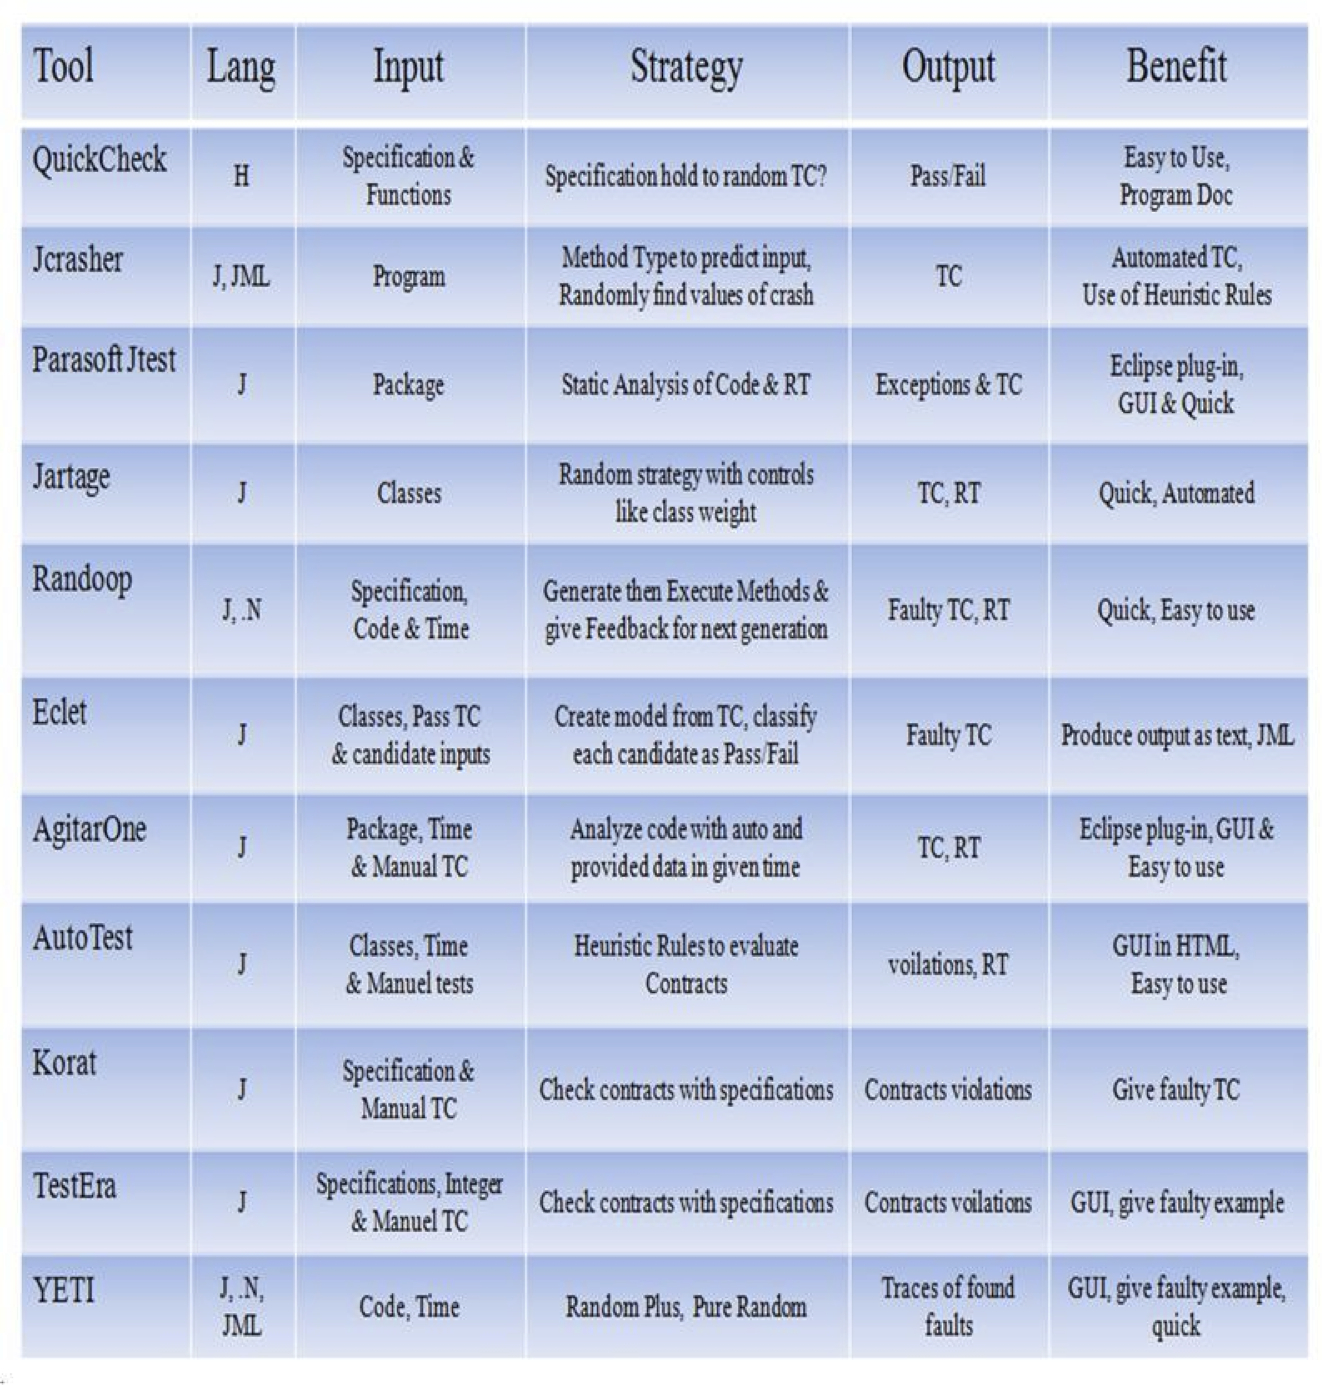
\includegraphics[scale=0.6]{Literature/tools}
	\caption{Summary of automated testing tools}
\end{figure}


\section{Conclusion}


% ------------------------------------------------------------------------


%%% Local Variables:
%%% mode: latex
%%% TeX-master: "../thesis"
%%% End:
